%% Los cap'itulos inician con \chapter{T'itulo}, estos aparecen numerados y
%% se incluyen en el 'indice general.
%%
%% Recuerda que aqu'i ya puedes escribir acentos como: 'a, 'e, 'i, etc.
%% La letra n con tilde es: 'n.

\chapter{Introducci\'on}
\label{Chapter1} % Change X to a consecutive number; for referencing this chapter elsewhere, use \ref{ChapterX}

%----------------------------------------------------------------------------------------
%	SECTION 1
%----------------------------------------------------------------------------------------


\section{Hidrogeles polim\'ericos: Aplicaciones biom\'edicas.} 

%%%%%%%%%%%%%%%%%%%%%%%%%%%%%%%%%%%%%%%%%
En la \'ultima d\'ecada, el inter\'es por los hidrogeles polim\'ericos ha aumentado significativamente debido a la amplia variedad y diversidad de materiales e innovaciones que se pueden lograr con ellos .
Estos sistemas polim\'ericos, que tienen una estructura molecular flexible y adaptable, pueden alterar su forma y propiedades de acuerdo con las condiciones externas.
Esta adaptabilidad los convierte en protagonistas indispensables en diversas industrias \cite{zhu2022review}, desde su uso en la creaci\'on de espumas y adhesivos \cite{wu2021review, chowdhury2019novel}, hasta su aplicaci\'on en la industria cosm\'etica y de pinturas, ofreciendo caracter\'isticas singulares a productos que enriquecen nuestra vida diaria \cite{hirst2019fundamentals}.
En la industria alimentaria, los hidrogeles polim\'ericos act\'uan como aditivos esenciales, contribuyendo a la textura, preservaci\'on y seguridad de los alimentos que consumimos \cite{kwok2019microgel}.

Los hidrogeles tienen aplicaciones significativas en la mejora de la retenci\'on de agua y nutrientes en el suelo, lo cual es fundamental para incrementar la productividad agr\'icola y disminuir la dependencia del riego \cite{el2004radiation}. Estos materiales tambi\'en son \'utiles en la protecci\'on de plantas contra sequ\'ias y plagas.
En el campo de la remediaci\'on ambiental, su capacidad para absorber y contener contaminantes es notable \cite{perez2018using,perez2019molecular}, contribuyendo as\'i a la purificaci\'on de agua y suelo \cite{mehrotra2021use}. Adem\'as, los hidrogeles facilitan el transporte y la liberaci\'on controlada de agentes remediadores, lo que acelera los procesos de limpieza ambiental \cite{mehrotra2021use}.
En resumen, los hidrogeles polim\'ericos se destacan por su versatilidad y su amplio espectro de aplicaciones pr\'acticas. Su habilidad para adaptarse a diversas condiciones ambientales los posiciona como herramientas valiosas en m\'ultiples sectores industriales.


 Uno de los terrenos m\'as importantes en los que los hidrogeles polim\'ericos han causado un impacto significativo es en el \'ambito m\'edico y farmac\'eutico. Estos materiales se han erigido como protagonistas en la b\'usqueda de transportadores de f\'armacos m\'as avanzados, eficientes, y compatibles con el organismo humano. Sus propiedades intr\'insecas les permiten ser moldeados y adaptados de manera espec\'ifica para cumplir con los requisitos \'unicos de la administraci\'on de medicamentos.
Esta capacidad permite dise\~nar hidrogeles  que se adapten a las necesidades espec\'ificas de cada paciente.
Esta intersecci\'on entre los hidrogeles polim\'ericos y la medicina no solo tiene el potencial de revolucionar la forma en que se administran medicamentos, sino que tambi\'en puede tener un impacto positivo en la calidad de vida de las personas. Se est\'an desarrollando tratamientos m\'as efectivos y personalizados que minimizan los efectos secundarios, gracias a la capacidad de estos materiales para interactuar de manera selectiva con el cuerpo humano. Adem\'as, lo degradable de estos materiales contribuye a la reducci\'on del impacto ambiental, lo que es fundamental en un mundo cada vez m\'as enfocado en la sostenibilidad.
La biodegradabilidad de los pol\'imeros que compones a estos hidrogeles permite que se eliminen del cuerpo de manera natural, evitando la necesidad de cirug\'ias para su extracci\'on \cite{samir2022recent}.

En aplicaciones m\'edicas los hidrogeles polim\'erico tienen  un creciente inter\'es. 
Como resultado, los hidrogeles de pol\'imeros son actualmente candidatos prometedores para el desarrollo de una variedad de biomateriales con aplicaciones en biosensores \cite{zhang2012ultrathin,islam2014responsive}, ingenier\'ia de tejidos \cite{matricardi2013interpenetrating,van2011biopolymer}, regeneraci\'on \'osea \cite{bai2018bioactive}, materiales biomim\'eticos \cite{green2016mimicking,wu2010multifunctional}, entre muchas otras aplicaciones biom\'edicas \cite{Daly2020}.
Por ejemplo, los films de  hidrogeles se pueden utilizar para crear parches transd\'ermicos que liberen f\'armacos de manera controlada y sostenida  \cite{indulekha2016thermoresponsive}.

Estos materiales se forman por la uni\'on de cadenas largas de mol\'eculas org\'anicas, es decir pol\'imeros, que pueden tener diferentes grados de entrecruzamiento y solvataci\'on. En la figura \ref{fig:intro:acidos-aa-maa} se ilustra c\'omo a partir de una cadena polim\'erica es posible crear una red de la misma y as\'i obtener un film o micro/nanogel. Estos pol\'imeros est\'an compuestos por mon\'omeros que son quienes otorgan sus cualidades est\'imulo-resposivas que resultan en sus multiples posibles aplicaciones.
Los films de hidrogeles son capas delgadas de material polim\'erico (redes tridimensionales entrecruzadas) con variados espesores depositadas o ancladas en superficies. Por otro lado, los microgeles son part\'iculas con una estructura de pol\'imero entrecruzado que, al igual que los films, pueden adsorber grandes cantidades de agua u otro solvente. Los nanogeles, en cambio, son estructuras similares a los microgeles pero de tama\~no nanom\'etrico.

En resumen, los hidrogeles polim\'ericos tienen un gran potencial para revolucionar una amplia gama de industrias, desde la cosm\'etica y alimenticia hasta la medicina y la farmac\'eutica. Su capacidad de adaptarse a diferentes condiciones y necesidades los convierte en una herramienta vers\'atil y valiosa para el desarrollo de nuevos productos y aplicaciones.



%%%%%%%%%%%%%%%%%%%%%%%%%%%%%%%

\section{Motivaci\'on: Encapsulado y Liberaci\'on de medicamentos}
%%%%%%%%%%%%%%%%%
%%%% Hirogeles y presentación de monomeros de trabajo
%%%%%%%%%%%%%%%%%

La naturaleza hidrof\'ilica de los hidrogeles los hace, generalmente, biocompatibles y poseen una gran capacidad para incorporar mol\'eculas hu\'esped o analitos, tanto org\'anicos como inorg\'anicos, y prevenir su degradaci\'on por el medio externo.
El ambiente acuoso dentro de las redes polim\'ericas puede proteger a las prote\'inas de la desnaturalizaci\'on y la agregaci\'on en el interior de los hidrogeles \cite{asayama2008comparison,sawada2010nano,beierle2014polymer}, mientras permanecen activas y estructuradas antes de ser liberadas \cite{vermonden2012hydrogels}. 
Como veh\'iculos para el suministro de drogas, los films y micro/nanogeles polim\'ericos pueden administrar f\'armacos de peso molecular bajo, oligonucle\'otidos, prote\'inas terap\'euticas e incluso combinaciones de drogas, lo cual es esencial en terapias contra el c\'ancer y las enfermedades infecciosas.
Estas aplicaciones son posibles gracias a su respuesta a est\'imulo que proporciona un mecanismo para el encapsulado y liberaci\'on de analitos.


La respuesta a est\'imulo de los films y micro/nanogeles est\'a fuertemente ligada a la composici\'on de los pol\'imeros que forman parte de su red tridimensional.
Los hidrogeles compuestos por cadenas polim\'ericas que contienen segmentos \'acidos como el \'acido acr\'ilico o metacr\'ilico (AA y MAA, respectivamente), suelen hincharse (swelling) o deshincharse (deswelling) en respuesta a cambios en el pH de la soluci\'on en la que se encuentran \cite{snowden1996colloidal}.
Esta respuesta al pH viene acompa\~nada con una regulaci\'on de carga por parte de la red polim\'erica, con lo que el material es tambi\'en capaz de responder simult\'aneamente a cambios en la concentraci\'on salina \cite{longo2019protonation}.
An\'alogamente, los hidrogeles compuestos por cadenas de pol\'imeros termosensibles experimentan una transici\'on de fase de volumen al sobrepasar una temperatura caracter\'istica \cite{Pelton1986,Pelton2000}.
Este comportamiento se origina porque tales pol\'imeros son insolubles en agua por encima de cierta temperatura m\'inima cr\'itica de solubilidad (LCST por sus siglas en ingl\'es) \cite{Kawaguchi2020}.
En particular, los hidrogeles compuestos por poli(N-isopropilacrilamida) (PNIPAm) poseen una LCST de alrededor de 32$^\circ$C \cite{Schild1992}.
En la figura \ref{fig:intro:acidos-aa-maa} se muestran ejemplos de mon\'omeros, cuyas cadenas polim\'ericas tienen este tipo de respuesta a cambios de  pH, concentraci\'on salina y/o temperatura. \'Acido metacr\'ilico (MAA) y  alilamina (AH) muestran respuesta al pH y a la concentraci\'on salina, el polim\'ero de  N-isopropilacrilamida (NIPAm)  presenta respuesta a la temperatura.
En esta tesis estudiaremos redes polim\'ericas compuestas con estos mon\'omeros, en particular se investiga si es posible utilizar sus hidrogeles polim\'ericos como dispositivos para aplicaciones biom\'edicas.  


\begin{figure*}[!htb]
	\centering
	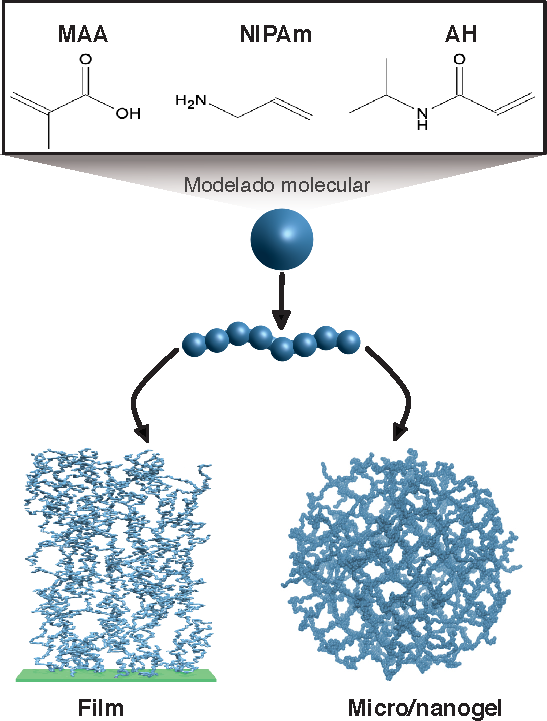
\includegraphics[width=0.75\linewidth]{Figures/modelos/hidrogeles.pdf}
	\caption{Mol\'eculas  que conforman los diferentes mon\'omeros de las redes polim\'ericas que dan respuesta a los hidrogeles. Con respuesta al pH y concentraci\'on de sal: alilamina (base),  \'acido metacr\'ilico y \'acido acr\'ilico. Con respuesta a la temperatura: N-isopropilacrilamida.
		Estas mol\'eculas son las utilizadas para los hidrogeles usados en esta tesis. Modelado molecular hace referencia a la construcci\'on  de modelos que representen las propiedades moleculares de estos sistemas. En particular se muestra que cada uno de estos mon\'omeros se presenta como una esfera. En cada cap\'itulo se dar\'a detalle de como se da la construcci\'on de este modelado. }
	\label{fig:intro:acidos-aa-maa}
\end{figure*}


%%%%%%%%%%%%%%%%%%%%%
%%%% respuesta al pH como estimulo para los carriers
%%%%%%%%%%%%%%%%%%
En la administraci\'on oral de f\'armacos, los hidrogeles con respuesta de pH se han investigado como veh\'iculos funcionales que pueden encapsular y administrar prote\'inas, evitando su degradaci\'on por el entorno gastrointestinal \cite{malmsten2010biomacromolecules,renukuntla2013approaches,koetting2014ph}. Esto se ilustra en la figura \ref{fig:intro:sistema}B en la que se muestran los cambios de pH que ocurren a lo largo del proceso digestivo, .


En este \'ambito, los cambios de pH presentes a lo largo del tracto digestivo, desde un medio \'acido en el est\'omago (pH 1.2-2) hasta uno neutro o moderadamente alcalino en el intestino delgado (pH 7-8), pueden ser aprovechados para controlar la liberaci\'on de f\'armacos.
Adem\'as, algunos compartimentos celulares involucrados en la captaci\'on de f\'armacos, como los endosomas tempranos, tienen un pH \'acido. La diferencia de pH que existe entre la superficie de la piel y el torrente sangu\'ineo puede ser aprovechada para la administraci\'on transd\'ermica de f\'armacos utilizando nanogeles con respuesta al pH \cite{qindeel2019development}.
Esto se ve esquematizado en la figura \ref{fig:intro:sistema}A en la cual se muestra c\'omo la respuesta a est\'imulo, pH  de los nanogeles funciona como agente liberador de drogas, en este caso por una expansi\'on de la part\'icula.
%A la derecha de la figura, se muestran los diferentes ambientes del tracto digestivo, en cuanto a valores de pH, con los cuales se pueden aprovechar los nanogeles con respuesta al pH.


\begin{figure}
	\centering
	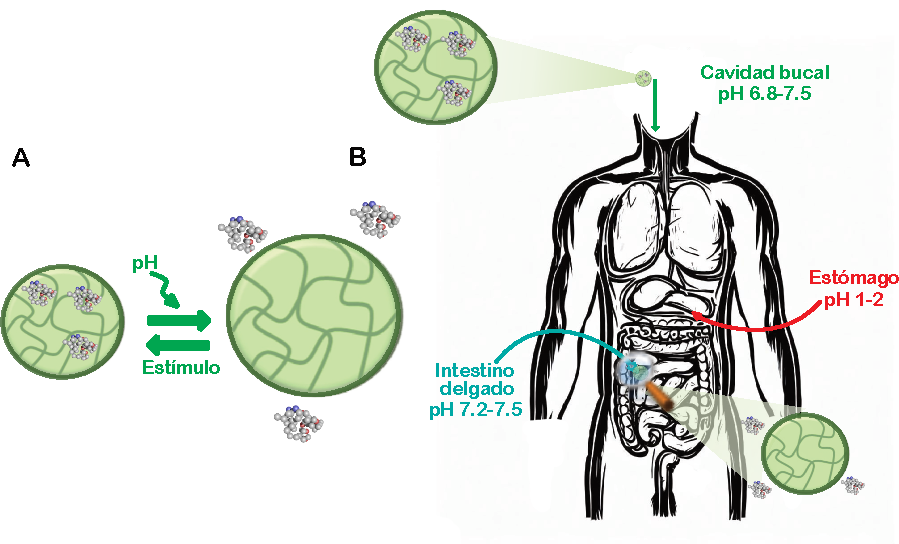
\includegraphics[width=0.99\textwidth]{Figures/modelos/sistema.pdf}
	\caption{Esquema de funcionamiento de nanogeles como transportadores de medicamentos. 
		\textbf{A} (izquierda): nanogel cargado con una prote\'ina terap\'eutica que se libera en respuesta a un est\'imulo (cambio de pH). \textbf{B} (lado derecho): se aprovecha los diferentes pHs que hay en el cuerpo humano para el dise\~no de nanogeles que liberen drogas terap\'euticas en un ambiente espec\'ifico. }
	\label{fig:intro:sistema}
\end{figure}

El microambiente local alrededor del tejido canceroso puede presentar un pH m\'as \'acido en comparaci\'on con las condiciones fisiol\'ogicas habituales \cite{lawson1963breast,tannock1989acid,gerweck2006tumor}, por lo que los nanogeles con respuesta al pH est\'an siendo evaluados para la administraci\'on de medicamentos en el tratamiento del c\'ancer \cite{peng2013controlled,kanamala2016mechanisms}. Por ejemplo, se han utilizado nanogeles de quitina para la administraci\'on de doxorubicina en diferentes tipos de c\'ancer, incluyendo pulm\'on, mama, h\'igado y pr\'ostata \cite{jayakumar2012doxorubicin}.

%%%%%%%%%%%%%%%
%%%%%  respuesta a T como estimulo para los carriers
%%%%%%%%%%%%%%

Por otro lado el pol\'imero termosensible, PNIPAm, al tener una temperatura de transici'on de volumen cercana a la temperatura corporal, hace que sus hidrogeles despierten un gran inter\'es para aplicaciones biom\'edicas, como la administraci\'on localizada de anest\'esicos \cite{Guan2011, indulekha2016thermoresponsive}. %%%% aqui
Es posible dise\~nar estrategias para controlar la temperatura de transici\'on de los hidrogeles termosensibles, las cuales incluyen la copolimerizaci\'on con un mon\'omero i\'onico o ionizable \cite{Cai2007,Macchione2019, Hirose1987,Lopez2020}.
Este \'ultimo enfoque produce hidrogeles de respuesta m\'ultiple que son susceptibles, adem\'as de a variaciones temperatura, a cambios en el pH y la concentraci\'on de sal.
En particular se ha demostrado que la temperatura de transici\'on de los microgeles de NIPAm y AA depende del pH de la soluci\'on y la concentraci\'on de sal \cite{Morris1997, Jones2000,Bradley2005,Begum2016}.
Asimismo la temperatura de transici\'on de los  microgeles de copol\'imeros de NIPAm y MAA \cite{Dowding2000,Hoare2004,Giussi2015} depende de la fracci\'on de mon\'omero ionizable en las cadenas de pol\'imero \cite{Morris1997,Jones2000, Hoare2004, Bradley2005, Lee2008,Wong2009,Hamzavi2016}.
Investigaciones recientes han explorado el uso de microgeles de poli(NIPAm-MAA) en dispositivos para la encapsulaci\'on y liberaci\'on del f\'armaco quimioterap\'eutico doxorrubicina \cite{Giussi2020, MartinezMoro2020, Pergushov2020}. La adici\'on de comon\'omero \'acido en estos microgeles introduce un nuevo mecanismo dependiente del pH para la captura y liberaci\'on eficiente de mol\'eculas, haciendo estos sistemas de microgeles multifuncionales especialmente prometedores para el dise\~no de sistemas avanzados de administraci\'on de f\'armacos \cite{Liu2017}.

En s\'intesis, el rango de las potenciales aplicaciones biom\'edicas de los nanogeles es extenso e incluye desarrollos contra los trastornos neurol\'ogicos, las enfermedades cardiovasculares, oftalmol\'ogicas, inflamatorias y autoinmunes, as\'i como tambi\'en avances en el diagn\'ostico por im\'agenes, la ingenier\'ia de tejidos, la reconstrucci\'on \'osea y el manejo de la diabetes y el dolor. Por ejemplo, los nanogeles de \'acido hialur\'onico est\'an siendo evaluados para inhibir la acumulaci\'on de la prote\'ina beta-amiloide en el manejo del Alzheimer \cite{jiang2018nanogels}. En el tratamiento de la diabetes, se investigan nanogeles sensibles a la glucosa \cite{wu2010multifunctional} y nuevos m\'etodos de administraci\'on de insulina basados en nanogeles \cite{nolan2004thermally}.

Estas son algunas razones por las cuales los hidrogeles polim\'ericos son hoy en d\'ia una de las primeras opciones consideradas al dise\~nar biomateriales con funciones espec\'ificas \cite{soni2016nanogels,sabir2019polymeric}. El est\'imulo que dispara la respuesta de los hidrogeles puede ser suministrado por un gradiente en la composici\'on fisiol\'ogica, ya sea natural o inducido por un estado patol\'ogico. La versatilidad de estas part\'iculas dif\'icilmente puede ser alcanzada con otro tipo de materiales incapaces de responder a cambios en las condiciones del medio que pueden ser relativamente moderados.
En este sentido uno de los desaf\'ios en la actualidad es aprender a controlar esta respuesta para canalizarla en diferentes aplicaciones. A lo largo de esta tesis se plantea comprender la fisicoqu\'imica, que determina el comportamiento de los hidrogeles polim\'ericos, en particular  films y micro/nanogeles, la cual determina su capacidad de responder a est\'imulos y como consecuencia su potencialidad para el desarrollo de dispositivos para el encapsulado y liberaci\'on de medicamentos.



%%%%%%%%
%%%% AFUERA
%Los mon\'omeros presentados en la figura \ref{fig:intro:acidos-aa-maa} tienen la particularidad de formar redes tridimensionales biodegradables y biocompatibles \cite{bajpai2008responsive}, lo que los hace atractivos para el dise\~no de biomateriales.




\section{Objetivos}

%%%%%%%%%%%%%%%%%%
El objetivo general de esta tesis es \textbf{desarrollar una descripci\'on comprensiva del comportamiento y respuesta a est\'imulos de los micro/nanogeles polim\'ericos mediante el uso de modelos te\'oricos y computacionales basados en interacciones moleculares.}

Este objetivo nos lleva a determinar si es posible utilizar hidrogeles polim\'ericos, ya sea en forma de films o micro/nanogeles, como dispositivos inteligentes para el desarrollo de nuevas tecnolog\'ias en biomedicina. En particular, el cap\'itulo \ref{Chapter-film} se dedica al estudio de films de hidrogeles polim\'ericos compuestos por mon\'omeros de \'acido metacr\'ilico, enfoc\'andose en la captura de poliaminas y la administraci\'on de drogas terap\'euticas, como la doxorubicina. Se analiza c\'omo interact\'uan estos films con diversas biomol\'eculas y/o drogas y c\'omo responden a cambios en el pH, concentraci\'on salina y concentraci\'on de adsorbatos, as\'i como los mecanismos subyacentes en la liberaci\'on de biomol\'eculas capturadas.
Para abordar estas cuestiones, desarrollamos un m\'etodo mecano-estad\'istico que denominamos Teor\'ia Molecular (TM).

En el cap\'itulo \ref{Chapter-geles}, se deriva una teor\'ia termodin\'amica para estudiar el comportamiento de microgeles de P(NIPAm-MAA) en respuesta a cambios de pH, concentraci\'on de sal y temperatura, se evalu\'a la actuaci\'on de estos microgeles para encapsular y liberar medicamentos en relaci\'on a las propiedades del medio. En el cap\'itulo \ref{Chapter-esfericas} se extiende la TM para investigar c\'omo la distribuci\'on del m\'onomero con respuesta al pH condiciona la adsorci\'on de prote\'inas terap\'euticas en nanogeles de PMAA y PAH.
Finalmente, el cap\'itulo \ref{chapter:mc:soluciones} aborda c\'omo los cambios en la concentraci\'on de nanogeles de P(NIPAm-MAA) afectan las propiedades de soluciones coloidales, en particular su respuesta al pH, concentraci\'on salina y temperatura. Para ello, integramos simulaciones de Monte Carlo con el modelo te\'orico desarrollado en el  cap\'itulo \ref{Chapter-geles}.


\section{Antecendentes metodol\'ogicos}\label{sec:intro:metodologicos}

%%%% Antecedentes TM
Mediante el uso de teor\'ia  molecular, se ha logrado estudiar la termodin\'amica de hidrogeles de cadenas de poli\'acido entrecruzadas, incluyendo pel\'iculas delgadas depositadas en superficies \cite{longo2012molecular,nap2006weak} y pel\'iculas  de estos mismos films anclados en superficies s\'olidas \cite{longo2014non,longo2014equilibrium}.
En estos trabajos, \citet{longo2014equilibrium} ha investigado el rol que cumple los cambios en el pH y la concentraci\'on de sal, en el equilibrio \'acido/base de poli\'acidos que componen al film. En otros trabajos se ha aplicado este marco te\'orico para considerar la adsorci\'on de p\'eptidos y prote\'inas en nanofilms de hidrogel de cadenas de poli\'acido entrecruzadas \cite{longo2014equilibrium,narambuena2015lysozyme,longo2016adsorption,hagemann2018use,szleifer1997protein,fang2005kinetics}, observando el trabajo no trivial que tiene el pH al momento de protonar/deprotonar a los distintos adsorbatos.

Las predicciones de esta teor\'ia han demostrado estar en excelente acuerdo cuantitativo con observaciones experimentales para una variedad de sistemas polim\'ericos \cite{tagliazucchi2010responsive,wu2007behavior}. En estos y otros trabajos se ha buscado comprender c\'omo la adsorci\'on en  pel\'iculas de hidrogel depende del pH y la concentraci\'on de sal, tanto en soluciones de prote\'inas individuales como en mezclas \cite{hagemann2018use,tagliazucchi2010responsive,longo2016adsorption}. En este m\'etodo, la TM, el estado de protonaci\'on de los residuos de prote\'inas y de los segmentos de la red no se asume a priori en funci\'on del pH de la soluci\'on (el seno o bulk), sino que se predice localmente como resultado de la posici\'on del grupo y su entorno local \cite{longo2019protonation,tagliazucchi2010responsive}.\\
%%%% pensar si sale o no...
%Estos resultados se lograron mediante la formulaci\'on de una energ\'ia libre general que incluye todas las contribuciones relevantes de estos sistemas polim\'ericos: el equilibrio \'acido-base, la p\'erdida entr\'opica de confinamiento molecular, los grados de libertad conformacionales de la red y las prote\'inas (o adsorbatos en general), y las interacciones electrost\'aticas, de Van der Waals y est\'ericas.


\section{Metodolog\'ia}

%%%%
\textbf{Teor\'ia Molecular}\\
En base a los antecendes metodol\'ogicos, los objetivos planteados en la presente tesis se abordaran principalmente con el desarrollo de una teor\'ia molecular con la cual poder describir la termodin\'amica de los sistemas de inter\'es.
Este enfoque te\'orico nos permite describir el tama\~no, la forma, la distribuci\'on de carga, el estado de protonaci\'on y la conformaci\'on de todas las especies moleculares que constituyen al sistema.  Para tal fin se usa una descripci\'on molecular de grano grueso de las diferentes especies qu\'imicas que componen el sistema. 

La TM se deriva al escribir la energ\'ia libre del sistema como un funcional de las densidades de las especies en soluci\'on, las conformaciones de la red polim\'erica y el potencial electrost\'atico.
%considerando expl\'icitamente los equilibrios \'acido-base.
La minimizaci\'on de esta energ\'ia respecto a los funcionales del sistema permite describir la termodin\'amica del sistema.
De esta manera, se puede estudiar c\'omo las variaciones en las condiciones de la soluci\'on: la fuerza i\'onica, el pH, la temperatura, concentraci\'on de alg\'un an\'alito de inter\'es, cambian las propiedades termodin\'amicas.

A lo largo de esta tesis se extiende la TM, en primera instancia, para el estudio de film de hidrogel  de poli\'acido para la captura de poliaminas, las cuales, como se demostrar\'a, funcionan como est\'imulo para la liberaci\'on de drogas terape\'uticas, en particular la doxorubicina (cap\'itulo \ref{Chapter-film}).
El uso de estos film en este cap\'itulo tuvo la finalidad de comprender los desarrollos te\'oricos planteados para los sistemas mencionados en los antecedentes metodol\'ogicos, secci\'on \ref{sec:intro:metodologicos}.
Comprendidas estas primeras bases, fue posible el estudio de la adsorci\'on de prote\'inas en nanogeles basados en PAH y PMAA, cap\'itulo \ref{Chapter-esfericas},  el cual necesit\'o de un nuevo desarrollo de teor\'ia molecular.
La complejidad de este nuevo estudio requiri\'o el uso de simulaciones por din\'amica molecular (DM)  para la obtenci\'on de las configuraciones de la red polim\'erica  los nanogeles.

%La teor\'ia molecular es un enfoque de funcional de la densidad en el cual los campos de interacci\'on se determinan  al considerar modelos detallados para cada uno de los componentes moleculares del sistema.
%Obtenemos la termodin\'amica que describe el sistema, adem\'as de informaci\'on estructural. 

%%%%%%%%%%%%%%%%%%%%%%%%%%%%%%%%
\textbf{Modelo termodin\'amico dos fases} \\
Se han descrito y aplicado teor\'ias y simulaciones moleculares en varios niveles de resoluci\'on para investigar el comportamiento de los hidrogeles polim\'ericos sensibles a est\'imulos.
\citet{quesada2011gel} han simulado el comportamiento de geles compuestos por polielectrolitos y termosensibles utilizando simulaciones de Monte Carlo, logrando explicar el comportamiento de hinchamiento de estas part\'iculas. Por otro lado, \citet{ahualli2016coarse} emplearon simulaciones de grano grueso para el modelado de geles polielectrol\'iticos. Estos trabajos se han centrado principalmente en el hinchamiento y otras propiedades de hidrogeles que tienen una red de pol\'imero permanentemente cargada. Algunos autores han tambi\'en abordado el efecto de la temperatura y la calidad del solvente \cite{Jha2011, QuesadaPerez2013, moncho-jorda2016a, ahualli2016coarse, AdroherBenitez2017PCCP}.

Recientemente, estudios mediante simulaciones cmputacionales han considerado la respuesta al pH de microgeles compuestos de pol\'imeros reguladores de carga \cite{Schroeder2015,Rud2017,Sean2018, Hofzumahaus2018,Lu2019}.
Sin embargo, solo unos pocos trabajos te\'oricos han investigado las propiedades de los microgeles de respuesta m\'ultiple en funci\'on de la temperatura, el pH y la concentraci\'on de sal \cite{CaprilesGonzalez2008,polotsky2013collapse}.

\citet{polotsky2013collapse} basa su teor\'ia en equilibrios osm\'oticos, teniendo en cuenta expl\'icitamente el equilibrio de ionizaci\'on dentro de sus microgeles. Estos estudios predicen patrones complejos en la dependencia de las dimensiones de las part\'iculas de microgel, es decir, sus par\'ametros de control: tama\~no y composici\'on.

En el cap\'itulo \ref{Chapter-geles} derivamos una teor\'ia de equilibrio entre dos fases y realizamos una investigaci\'on sistem\'atica del comportamiento termodin\'amico de microgeles compuestos por copol\'imeros aleatorios de NIPAm y un comon\'omero \'acido, MAA. Este modelo describe la qu\'imica-f\'isica detr\'as de diversos fen\'omenos: a saber la expansi\'on del microgel impulsada por el pH, la dependencia del tama\~no de part\'icula en la concentraci\'on de sal, y el efecto de los cambios en la temperatura. La finalidad de esta metolog\'ia es obtener las condiciones, dado el pH, temperatura, concentraci\'on salina, y tama\~no del microgel, que minimizan la energ\'ia  del sistema. Esto se logra a  trav\'es de escribir un potencial termodin\'amico que incluya las diferentes contribuciones que hacen al sistema: entrop\'ia de mezcla, energ\'ia libre qu\'imica de las especies protonables, energ\'ia asociada a interacciones electrost\'aticas y del tipo Van der Waals, as\'i  como tambi\'en por las repulsiones est\'ericas.  


%%%%%%%%%%%%%%%%%%%%%%%%%%%%%%%%
%%%%%%%%%%%%%%%%%%%%%%%%%%%%%%%%%%%%%%%%%%%%%%%%%%%%%%


\textbf{Metr\'opolis Monte Carlo}\\
El m\'etodo de Metropolis Monte Carlo (MCMC) es un m\'etodo de muestreo estad\'istico que se utiliza para generar muestras de una distribuci\'on de probabilidad desconocida. El m\'etodo es utilizado en el cap\'itulo \ref{chapter:mc:soluciones} para el estudio de soluciones coloidales de nanogeles basados en P(NIPAm-MAA). En cada paso de estas simulaciones un nanogel de la soluci\'on es seleccionado al azar cambiandolo de posici\'on en la soluci\'on seguido de una expansi\'on/compresi\'on del mismo.
La probabilidad de aceptar o no este paso es mediado por la energ\'ia total del paso: energ\'ia interna del nanogel y energ\'ia de interacci\'on con los dem\'as nanogeles presentes en la soluci\'on. La energ\'ia interna de estos nanogeles es la energ\'ia libre interna obtenida con la metodolog\'ia del modelo termodin\'amico de dos fases presentada en el cap\'itulo \ref{Chapter-geles}. 
En este cap\'itulo se desarrolla el estudio de las propiedades coloidales de los soluciones de nanogeles y como se ven afectadas a consecuencia de la composici\'on de la soluci\'on, pH, concentraci\'on de sal o por la temperatura a la cual se encuentra la misma.


%\textbf{Din\'amica Molecular}\\

%La din\'amica molecular (MD) es una t\'ecnica computacional que permite estudiar el comportamiento de las mol\'eculas a trav\'es del tiempo. Esta t\'ecnica simula el movimiento de los \'atomos que componen las mol\'eculas, y permite observar c\'omo las mol\'eculas interact\'uan entre s\'i y con su entorno.
%GROMACS es un software de c\'odigo abierto que se utiliza para realizar simulaciones de din\'amica molecular. \cite{lindahl2001gromacs}
%El paquete de simulaci\'on GROMACS es ampliamente utilizado para llevar a cabo simulaciones de din\'amica molecular en sistemas biol\'ogicos, qu\'imicos y materiales. Su capacidad para modelar la interacci\'on entre part\'iculas y representar fuerzas realistas permite el estudio de sistemas complejos y la obtenci\'on de resultados cuantitativos y cualitativos significativos.

%Esta metodolog\'ia se ha usado en conjunto de la teor\'ia molecular, en particulas las simulaciones de DM se han utilizado para la generaci\'on de configuraciones  de la red polim\'erica de los hidrogeles de estudio. Se describe la confecci\'on de las configuraciones para un nanogel polim\'erico en el anexo \ref{anexo-configuraciones}.





%%%%%%%%%%%%%%%%%recorte
%%%%%%%%%%%%%%%%%%%%


%-----------------------------------
%	SUBSECTION 1
%-----------------------------------





